\section{Video Understanding: Thị giác Vượt qua Thời gian}
\label{sec:video_understanding}

\subsection{Giới thiệu: Khi Ảnh bắt đầu Chuyển động}
\label{subsec:video_intro}

Tất cả các chương trước của cuốn sách này—từ CNN đến Transformer, từ object detection đến segmentation—đều hoạt động trên \textit{ảnh tĩnh}. Nhưng thế giới thực tồn tại trong thời gian. Một bức ảnh chụp người đang chạy trông hệt như một bức ảnh người đang đứng khom người. Chỉ khi xem nhiều khung hình liên tiếp, chúng ta mới hiểu được hành động đang diễn ra.

Video không chỉ là một tập hợp ảnh rời rạc. Nó là dữ liệu \textbf{không-thời gian (spatiotemporal)}: mỗi khung hình mang thông tin không gian, và \textit{chuỗi} các khung hình mang thông tin thời gian — chuyển động, nhịp điệu, nhân quả.

\begin{mdframed}[style=infobox]
    \textbf{Thách thức đặc trưng của Video}
    \begin{itemize}
        \item \textbf{Chiều thời gian:} Mô hình phải "nhớ" những gì đã xảy ra ở các khung trước để hiểu khung hiện tại.
        \item \textbf{Khối lượng dữ liệu khổng lồ:} Video 30fps $\times$ 1280$\times$720 $\times$ 3 kênh = hàng trăm MB mỗi phút. Xử lý hiệu quả là bắt buộc.
        \item \textbf{Chuyển động dài hạn:} Nhận ra hành động "bơi" đòi hỏi hiểu chuyển động diễn ra trong nhiều giây, không phải vài khung hình.
    \end{itemize}
\end{mdframed}

\subsection{Two-Stream Networks: Ảnh và Chuyển động Song hành}
\label{subsec:two_stream}

\subsubsection{Ý tưởng: Hai luồng thông tin bổ trợ}
\label{subsubsec:two_stream_idea}

Simonyan và Zisserman (2014) \cite{Simonyan2014} đề xuất một kiến trúc hai luồng (two-stream) lấy cảm hứng từ khoa học thần kinh: hệ thống thị giác linh trưởng có hai con đường xử lý — \textit{ventral stream} (nhận dạng vật thể) và \textit{dorsal stream} (nhận thức chuyển động).

\begin{enumerate}
    \item \textbf{Spatial Stream:} Nhận đầu vào là một khung hình RGB đơn lẻ, học nhận dạng ngữ cảnh và đối tượng (ai đang làm gì, ở đâu).
    \item \textbf{Temporal Stream:} Nhận đầu vào là \textit{stacked optical flow fields} (ví dụ: 10 khung liên tiếp của $(u, v)$ flow, tổng cộng 20 kênh), học nhận dạng chuyển động và tốc độ.
\end{enumerate}

Hai luồng được huấn luyện riêng rẽ và kết hợp bằng late fusion (ghép softmax scores).

\begin{center}
    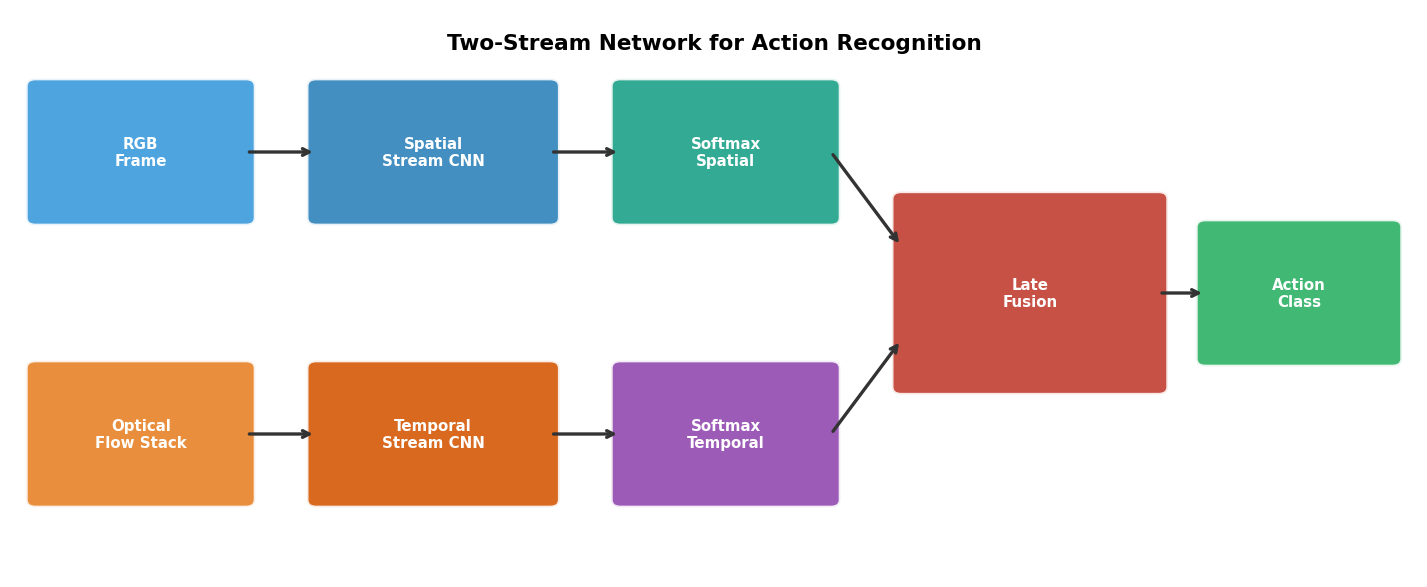
\includegraphics[width=0.9\textwidth]{images/two_stream_network.png}
    \captionof{figure}{Kiến trúc Two-Stream Network. Luồng không gian (spatial stream) xử lý ảnh RGB; luồng thời gian (temporal stream) xử lý optical flow. Hai luồng được kết hợp ở cuối để phân loại hành động.}
    \label{fig:two_stream_network}
\end{center}

Two-Stream Network đặt nền móng quan trọng: optical flow là "ngôn ngữ chuyển động" tự nhiên cho video recognition. Hạn chế là optical flow tốn kém để tính, và hai luồng không chia sẻ thông tin trong quá trình xử lý.

\subsection{3D CNNs: Tích chập trong Không-Thời gian}
\label{subsec:3d_cnn}

\subsubsection{C3D: Tích chập 3D thuần túy}
\label{subsubsec:c3d}

Nếu ảnh 2D được xử lý bằng kernel 2D ($H \times W$), tại sao không xử lý video bằng kernel \textit{3D} ($T \times H \times W$) để đồng thời trích xuất đặc trưng không gian và thời gian?

\textbf{C3D} \cite{Tran2015} (2015) là kiến trúc 3D CNN đầu tiên hoạt động hiệu quả ở quy mô lớn. Nó sử dụng các kernel $3 \times 3 \times 3$ (thời gian $\times$ chiều cao $\times$ chiều rộng) và được huấn luyện trên Sports-1M, tập video lớn nhất thời bấy giờ.

\subsubsection{I3D: Inflated 3D Networks}
\label{subsubsec:i3d}

\textbf{I3D} \cite{Carreira2017} (2017) đề xuất một ý tưởng cực kỳ thực dụng: "thổi phồng" (inflate) các kernel 2D đã được pre-train trên ImageNet thành kernel 3D bằng cách sao chép theo chiều thời gian.

Một kernel 2D $k \times k$ được biến thành kernel 3D $t \times k \times k$, và các trọng số được sao chép $t$ lần rồi chia cho $t$ để giữ nguyên giá trị kỳ vọng. Điều này cho phép tận dụng toàn bộ kiến thức đã học từ ImageNet—thay vì khởi tạo ngẫu nhiên.

I3D kết hợp với kiến trúc Two-Stream (I3D spatial + I3D temporal) đạt kết quả tốt nhất trên UCF101 và Kinetics tại thời điểm ra mắt.

\subsection{SlowFast Networks: Nhìn Chậm và Nhìn Nhanh}
\label{subsec:slowfast}

\textbf{SlowFast} \cite{Feichtenhofer2019} (2019) của Feichtenhofer và cộng sự (Facebook AI) đưa ra một triết lý xử lý video hoàn toàn mới, lấy cảm hứng từ hệ thống tế bào thần kinh thị giác:

\begin{itemize}
    \item Trong võng mạc người, ~80\% tế bào thần kinh là \textit{tế bào P (Parvocellular)}: phản hồi \textit{chậm}, nhạy với màu sắc và chi tiết không gian.
    \item ~20\% còn lại là \textit{tế bào M (Magnocellular)}: phản hồi \textit{nhanh}, nhạy với chuyển động.
\end{itemize}

Kiến trúc SlowFast hiện thực hóa điều này:

\begin{enumerate}
    \item \textbf{Slow Pathway:} Xử lý video ở \textit{tần suất khung hình thấp} (ví dụ: 4fps), với \textit{nhiều kênh}. Chuyên về học ngữ nghĩa không gian và đặc trưng ngoại hình.
    \item \textbf{Fast Pathway:} Xử lý video ở \textit{tần suất cao} (ví dụ: 32fps), với \textit{ít kênh} hơn nhiều ($\approx 1/8$). Chuyên về học chuyển động tốc độ cao.
    \item \textbf{Lateral Connections:} Hai pathway được kết nối ở nhiều thời điểm để trao đổi thông tin.
\end{enumerate}

\begin{center}
    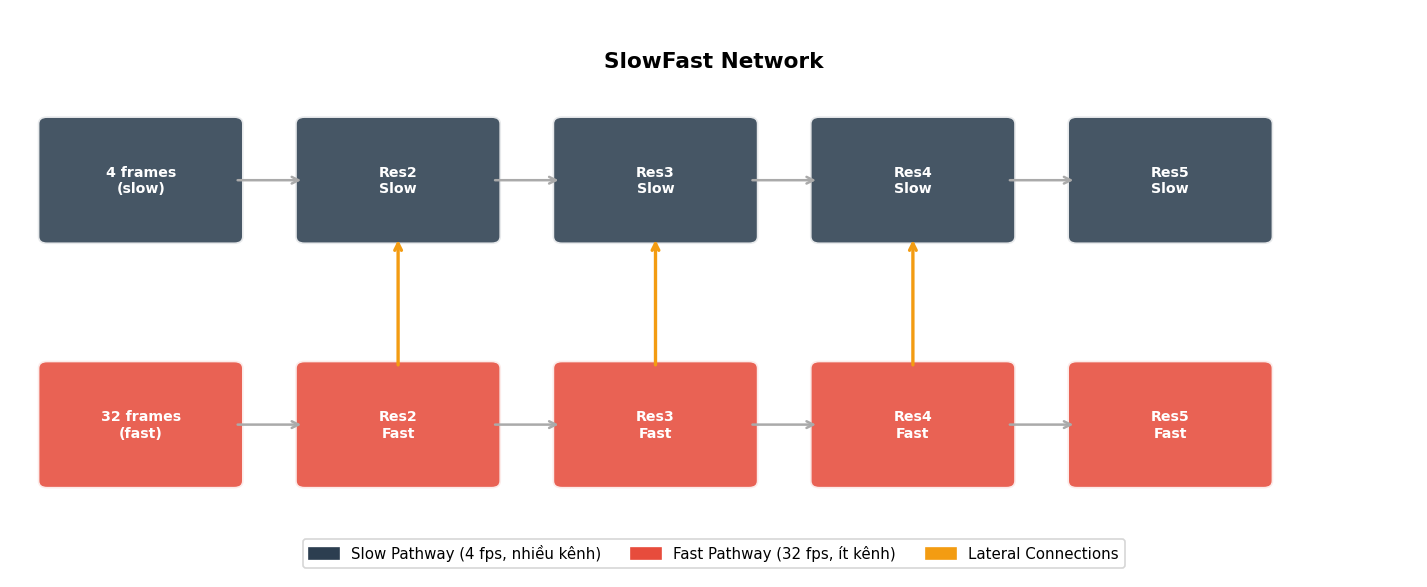
\includegraphics[width=1.0\textwidth]{images/slowfast_network.png}
    \captionof{figure}{Kiến trúc SlowFast. Slow pathway (trên) xử lý ít khung hình nhưng nhiều kênh đặc trưng, học ngữ nghĩa. Fast pathway (dưới) xử lý nhiều khung hình hơn nhưng ít kênh hơn, học chuyển động. Các kết nối ngang (lateral connections) kết nối hai pathway.}
    \label{fig:slowfast_network}
\end{center}

SlowFast không những đạt state-of-the-art mà còn hiệu quả hơn 3D CNN đơn thuần, vì Fast pathway rất gọn nhẹ.

\subsection{Video Transformers: Self-Attention trong Không-Thời gian}
\label{subsec:video_transformers}

Sự ra đời của Vision Transformer tất nhiên dẫn đến việc mở rộng sang video. Thách thức chính: một video $T$ khung hình, mỗi khung $H \times W$ pixel, bị chia thành các patch sẽ tạo ra một chuỗi dài khổng lồ — self-attention có độ phức tạp $O(n^2)$.

\textbf{TimeSformer} \cite{Bertasius2021} (2021) giải quyết bằng \textit{divided space-time attention}: thay vì attention toàn cục, tính riêng biệt:
\begin{itemize}
    \item \textit{Spatial Attention}: mỗi patch chú ý đến các patch khác trong cùng khung hình.
    \item \textit{Temporal Attention}: mỗi patch chú ý đến cùng vị trí không gian đó ở các khung hình khác.
\end{itemize}

\textbf{Video Swin Transformer} \cite{Liu2022video} mở rộng Swin Transformer sang 3D với cửa sổ trượt trong không-thời gian, cho phép xử lý video dài hiệu quả hơn.

\subsection{Bài toán Action Recognition: Benchmark Video Understanding}
\label{subsec:action_recognition}

\textbf{Action Recognition} (nhận dạng hành động) là bài toán chuẩn (benchmark) của video understanding: cho một đoạn video ngắn, phân loại hành động đang diễn ra (chạy, nhảy, bơi, nấu ăn...).

Các tập dữ liệu benchmark chính:
\begin{itemize}
    \item \textbf{UCF101, HMDB51:} Các tập cổ điển, quy mô nhỏ, nay đã bão hòa.
    \item \textbf{Kinetics-400/600/700:} Tập lớn nhất, được thu thập từ YouTube, là benchmark tiêu chuẩn cho các mô hình hiện đại.
    \item \textbf{AVA:} Tập phức tạp hơn, yêu cầu nhận biết hành động tại vị trí cụ thể (spatiotemporal action detection).
\end{itemize}

\begin{table}[h!]
    \centering
    \caption{So sánh các kiến trúc Video Understanding theo thời gian}
    \label{tab:video_arch_comparison}
    \begin{tabular}{|l|l|p{4.5cm}|l|}
        \hline
        \textbf{Kiến trúc} & \textbf{Năm} & \textbf{Ý tưởng chính} & \textbf{Đặc điểm} \\
        \hline
        Two-Stream & 2014 & RGB + Optical Flow riêng biệt & Cần tính flow tốn kém \\
        C3D & 2015 & Tích chập 3D thuần túy & Nặng, nhiều tham số \\
        I3D & 2017 & Inflate 2D CNN từ ImageNet & Hiệu quả pretrain \\
        SlowFast & 2019 & Hai pathway chậm/nhanh & Cân bằng tốt \\
        TimeSformer & 2021 & Divided space-time attention & Không cần conv \\
        Video Swin & 2022 & Swin 3D với shifted windows & Linh hoạt, hiệu quả \\
        \hline
    \end{tabular}
\end{table}

\begin{mdframed}[style=infobox]
    \textbf{Kết nối với Chương 9 (Multimodal)}

    Video Understanding là nền tảng không thể thiếu để hiểu các Video-Language Models sẽ được trình bày trong chương tiếp theo. Các mô hình như VideoCLIP, VideoChat, hay các tính năng video của GPT-4o đều dựa trên khả năng trích xuất đặc trưng từ video mà chúng ta vừa học ở đây. Chuyển động trong video không chỉ là chuỗi ảnh—nó là ngôn ngữ của thế giới vật lý, và hiểu được nó là bước cơ bản để AI có thể lý luận về thực tế.
\end{mdframed}

\section*{Tài liệu tham khảo}
\begin{itemize}
    \item[1] Simonyan, K.; Zisserman, A. Two-Stream Convolutional Networks for Action Recognition in Videos. In \textit{NeurIPS}, 2014.
    \item[2] Tran, D. et al. Learning Spatiotemporal Features with 3D Convolutional Networks (C3D). In \textit{ICCV}, 2015.
    \item[3] Carreira, J.; Zisserman, A. Quo Vadis, Action Recognition? A New Model and the Kinetics Dataset (I3D). In \textit{CVPR}, 2017.
    \item[4] Feichtenhofer, C. et al. SlowFast Networks for Video Recognition. In \textit{ICCV}, 2019.
    \item[5] Bertasius, G. et al. Is Space-Time Attention All You Need for Video Understanding? (TimeSformer). In \textit{ICML}, 2021.
    \item[6] Liu, Z. et al. Video Swin Transformer. In \textit{CVPR}, 2022.
\end{itemize}
